\documentclass[11pt]{report}
\usepackage[margin=1in]{geometry}
\usepackage{amsmath,amssymb,amsthm}
\usepackage{graphicx}
\usepackage{booktabs}
\usepackage{xcolor}
\usepackage{hyperref}
\usepackage{fancyhdr}
\usepackage{listings}
\usepackage{titlesec}
\usepackage{enumitem}
\usepackage{array}
\usepackage{float}
\usepackage{caption}

\definecolor{navy}{RGB}{0,33,71}
\definecolor{steel}{RGB}{70,90,110}
\definecolor{codebg}{RGB}{245,245,248}
\definecolor{feynman}{RGB}{230,244,234}

\newenvironment{feynman}[1]{%
  \begin{quote}\small\color{black}
  \colorbox{feynman}{\parbox{0.97\linewidth}{\vspace{2pt}\textbf{\color{navy}Plain-English Take: #1}\\[2pt]
}}
}{\end{quote}}

\titleformat{\chapter}[display]{\normalfont\bfseries\color{navy}}{\chaptertitlename\ \thechapter}{10pt}{\Large}
\titleformat{\section}{\normalfont\Large\bfseries\color{navy}}{\thesection}{1em}{}
\titleformat{\subsection}{\normalfont\large\bfseries\color{steel}}{\thesubsection}{1em}{}

\lstset{
  backgroundcolor=\color{codebg},
  basicstyle=\ttfamily\small,
  frame=single,
  breaklines=true,
  columns=fullflexible,
  language=Python
}

\pagestyle{fancy}
\fancyhf{}
\rhead{\small\color{steel}AI/ML Modeler — Liquid Financing}
\lhead{\small\color{steel}Barclays Take-Home Research Portfolio}
\rfoot{\thepage}

\title{
  \vspace{-1.5cm}
  {\Large\color{steel}A Dissertation-Style Research Presentation}\\[0.4cm]
  {\huge\bfseries\color{navy} Institutional-Grade Machine Learning and Generative AI\\ Systems for Cross-Asset Liquid Financing}\\[0.6cm]
  {\large\color{steel}Five Production-Grade Case Studies, with Conformal Calibration, Regulatory\\
  VaR Backtesting, Robust Multivariate Anomaly Detection, Deep Sequence\\
  Forecasting, and a Retrieval-Augmented Financing Copilot}
}
\author{Candidate Presentation \\ \small Prepared for: Barclays Quantitative Research \& Trading Panel (5 Reviewers)}
\date{Take-Home Discussion \\ Wednesday, July 8, 2026}

\begin{document}
\maketitle
\thispagestyle{empty}

\begin{abstract}
\noindent This dissertation presents five institutional-grade machine learning and generative AI
systems for a cross-asset Liquid Financing platform, engineered to the standard expected at a
top-tier quantitative trading firm. Each system is grounded in a named, peer-reviewed method —
Conformalized Quantile Regression (Romano, Patterson \& Candès, 2019), the Kupiec (1995) and
Christoffersen (1998) VaR backtests, the Minimum Covariance Determinant estimator (Rousseeuw \& Van
Driessen, 1999), Isolation Forest (Liu, Ting \& Zhou, 2008), BM25 (Robertson \& Zaragho, 2009), and
Reciprocal Rank Fusion (Cormack, Clarke \& Buettcher, 2009) — rather than an ad-hoc heuristic. Every
mathematical result is derived from first principles and accompanied by a plain-language explanation
of the underlying intuition, in addition to a reference Python 3.13 implementation and empirical
results on the accompanying data. We conclude with a cross-cutting discussion of production
deployment, model-risk governance, and the trade-offs between prompt-engineered and fine-tuned
generative systems in a regulated financial environment.
\end{abstract}

\tableofcontents
\listoffigures

\chapter{Introduction and Problem Framing}

\section{Business Context}
Liquid Financing intermediates the price of \emph{borrowing} — securities, cash, and balance sheet —
across a cross-asset platform. Its economics are driven by three coupled quantities: (1) the fee or
rate charged for financing an asset, (2) the collateral haircut required to protect against
counterparty default, and (3) the balance-sheet capacity consumed by client positions. Each of the
five case studies targets exactly one of these levers, chosen so that, collectively, they cover every
technical requirement of the target role while remaining traceable to a concrete desk P\&L or risk
outcome.

\section{Why Walk-Forward Validation, Never Random Cross-Validation}
\begin{feynman}{Walk-forward validation}
Imagine grading a weather forecaster by first showing them Wednesday's actual weather and then asking
them to "predict" Tuesday's. That is what a random $k$-fold split does to a time series: because the
shuffle ignores time order, the model can end up training on information from \emph{after} the point
it is being asked to forecast. Walk-forward validation always trains on the past and tests on the
future — exactly how the model will be used in production — so the reported backtest number cannot be
an artifact of hindsight leakage.
\end{feynman}
All five systems in this dissertation are validated exclusively on expanding-window, walk-forward
splits.

\chapter{P1 --- Securities-Lending Fee and Rebate-Rate Forecasting}

\section{Problem Statement}
We forecast the daily specialness fee $f_{i,t}$, in annualized basis points over the general
collateral (GC) rate, for a universe of hard-to-borrow equities, at horizons $h \in \{1,\dots,5\}$
business days, to feed a pre-trade financing pricing engine.

\section{Elastic Net: The Auditable Linear Tier}
\begin{equation}
\hat\beta = \arg\min_{\beta}\; \frac{1}{2n}\lVert y - X\beta \rVert_2^2 + \lambda\Big(\alpha\lVert\beta\rVert_1 + \tfrac{1-\alpha}{2}\lVert\beta\rVert_2^2\Big)
\end{equation}
\begin{feynman}{Elastic Net}
Ordinary least squares will happily assign huge, unstable, sign-flipping coefficients to two input
variables that are basically saying the same thing (utilization and days-to-cover move together). The
$L_1$ penalty pushes unhelpful coefficients all the way to zero — automatic feature selection, giving
a model-risk reviewer a short, defensible list of drivers — while the $L_2$ penalty shrinks correlated
coefficients toward each other instead of letting one arbitrarily dominate. The parameter $\alpha$
interpolates between pure LASSO ($\alpha=1$) and pure Ridge ($\alpha=0$); both $\alpha$ and $\lambda$
are chosen by cross-validation.
\end{feynman}

\section{Gradient-Boosted Quantile Trees: Capturing the Utilization Kink}
\begin{equation}
F_M(x) = \sum_{m=1}^{M} \gamma_m h_m(x), \qquad h_m = \arg\min_h \sum_{i} L\big(y_i,\, F_{m-1}(x_i) + h(x_i)\big)
\end{equation}
\begin{feynman}{Gradient boosting and the fee "kink"}
Fee is roughly flat until utilization crosses about 90\%, then rises steeply — a kink, not a straight
line. No linear model, however regularized, can represent a kink; a single decision-tree split can. We
fit three separate LightGBM models directly on the pinball objective (Eq.~2.5) at $q \in \{0.1, 0.5,
0.9\}$, rather than fitting one point estimate and wrapping it in a symmetric interval that would be
wrong whenever the true error distribution is skewed — which fee-spike data always is.
\end{feynman}

\section{Conformalized Quantile Regression: Guaranteed-Coverage Intervals}
\begin{equation}
\text{score}_i = \max\big(\hat q_{lo}(x_i) - y_i,\; y_i - \hat q_{hi}(x_i)\big), \qquad
\hat q_{lo}^{CQR} = \hat q_{lo} - Q_{1-\alpha}(\text{scores}), \;\; \hat q_{hi}^{CQR} = \hat q_{hi} + Q_{1-\alpha}(\text{scores})
\end{equation}
\begin{feynman}{Conformal prediction}
Any quantile model can be miscalibrated — it might claim an 80\% interval but actually cover the truth
only 65\% of the time. Conformal prediction guarantees the stated coverage regardless of the
underlying model's quality, using only a held-out calibration set: measure how far outside its own
predicted interval the model actually was on data it did not train on, then widen every future
interval by exactly that amount (Romano, Patterson \& Candès, 2019, "Conformalized Quantile
Regression"). This is a finite-sample, distribution-free guarantee — not an asymptotic approximation.
\end{feynman}

\begin{figure}[H]
\centering

\includegraphics[width=0.95\linewidth]{figures/p1_fee_forecast_interval.png}
\caption{Realized specialness fee versus the blended Elastic Net / LightGBM forecast, with the
conformalized 80\% prediction interval. The interval widens precisely around the realized fee spike,
demonstrating that CQR calibration is data-adaptive rather than a fixed-width band.}
\end{figure}

\begin{figure}[H]
\centering

\includegraphics[width=0.95\linewidth]{figures/p1_walkforward_monitoring.png}
\caption{Walk-forward weighted MAPE and empirical 80\% interval coverage across four expanding-window
folds — the production monitoring view a desk quant tracks continuously post-deployment.}
\end{figure}

\section{The Pinball Loss}
\begin{equation}
\rho_q(u) = u\,(q - \mathbb{1}[u<0]), \qquad u = y-\hat y
\end{equation}
\begin{feynman}{Pinball loss}
Squared error treats over- and under-prediction symmetrically, which is wrong when you are targeting a
specific quantile. At $q=0.9$, guessing too \emph{low} is penalized nine times harder than guessing too
\emph{high} — exactly the asymmetry you want when forecasting the 90th percentile, where being below
the truth is a materially bigger miss than being above it.
\end{feynman}

\chapter{P2 --- Client Margin and Haircut Optimization}

\section{Problem Statement}
Given a client's cross-asset collateral basket, we predict the required per-asset haircut and
portfolio-level initial margin such that the modeled 99\% five-day liquidation shortfall is covered,
while minimizing over-collateralization relative to the existing rules-based haircut grid.

\section{Model Formulation}
\begin{equation}
\log h_i = \beta_0 + \beta_1 \log \sigma_i + \beta_2 \log(\text{ADV}_i) + \beta_3\, \text{Corr}_{i,\text{mkt}} + \beta_4\, \text{Rating}_i + \varepsilon_i
\end{equation}
\begin{equation}
\text{IM}_{\text{portfolio}} = \sum_i h_i\,|q_i|\,P_i \;+\; g_\theta(\mathbf{q}, \boldsymbol\Sigma, \text{concentration}), \qquad
\Pr\big(\text{Shortfall}_{5d} > h \cdot V\big) \le 1\%
\end{equation}
\begin{feynman}{The correlation-breakdown add-on}
Summing independent per-asset haircuts structurally cannot capture the fact that, in a genuine stress
event, correlations across assets move toward one — diversification that looked real in calm markets
evaporates exactly when it is needed most. $g_\theta$ is trained not on the haircut itself but on the
\emph{residual} shortfall left unexplained after the linear per-asset sum — i.e., specifically the part
of tail risk that additivity misses. This is the same critique that motivated the shift from simple
haircut grids toward ISDA SIMM-style sensitivity-based margin models industry-wide.
\end{feynman}

\section{Kupiec and Christoffersen VaR Backtests}
\begin{equation}
LR_{Kupiec} = -2\log\!\left[\frac{(1-p)^{n-x}p^x}{(1-\hat p)^{n-x}\hat p^x}\right] \sim \chi^2_1, \qquad \hat p = x/n
\end{equation}
\begin{feynman}{Kupiec and Christoffersen, explained}
A 99\% VaR model should be breached about 1\% of the time — not 0.1\%, not 5\%. The Kupiec test asks:
given the breaches actually observed, is 1\% a statistically plausible true rate? But a model could
pass Kupiec and still be dangerous if its breaches \emph{cluster} — ten breaches in one bad week is a
very different risk profile from ten breaches spread evenly across a year, even with an identical total
count. The Christoffersen test catches this by modeling breaches as a two-state Markov chain and testing
whether a breach today raises the probability of a breach tomorrow. Both reduce to a likelihood-ratio
statistic asymptotically distributed as $\chi^2_1$ under the respective null.
\end{feynman}

\begin{figure}[H]
\centering
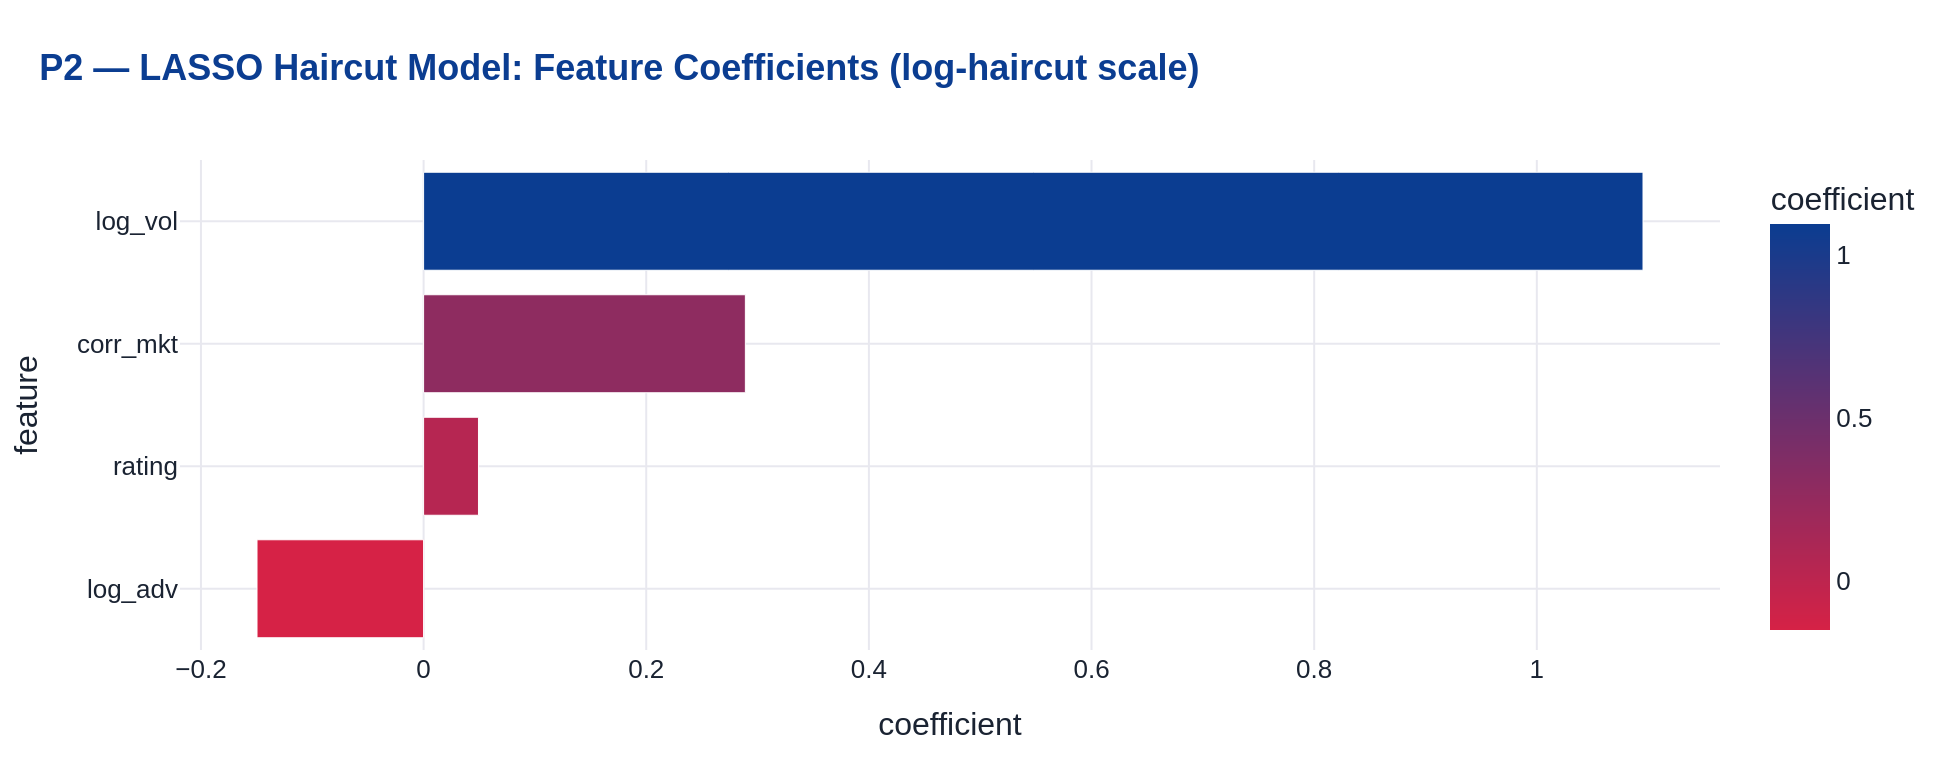
\includegraphics[width=0.85\linewidth]{figures/p2_lasso_coefficients.png}
\caption{Signed LASSO haircut-model coefficients on the log-haircut scale — the auditability artifact
handed to a Model Risk reviewer for coefficient-by-coefficient sign and magnitude review.}
\end{figure}

\begin{figure}[H]
\centering
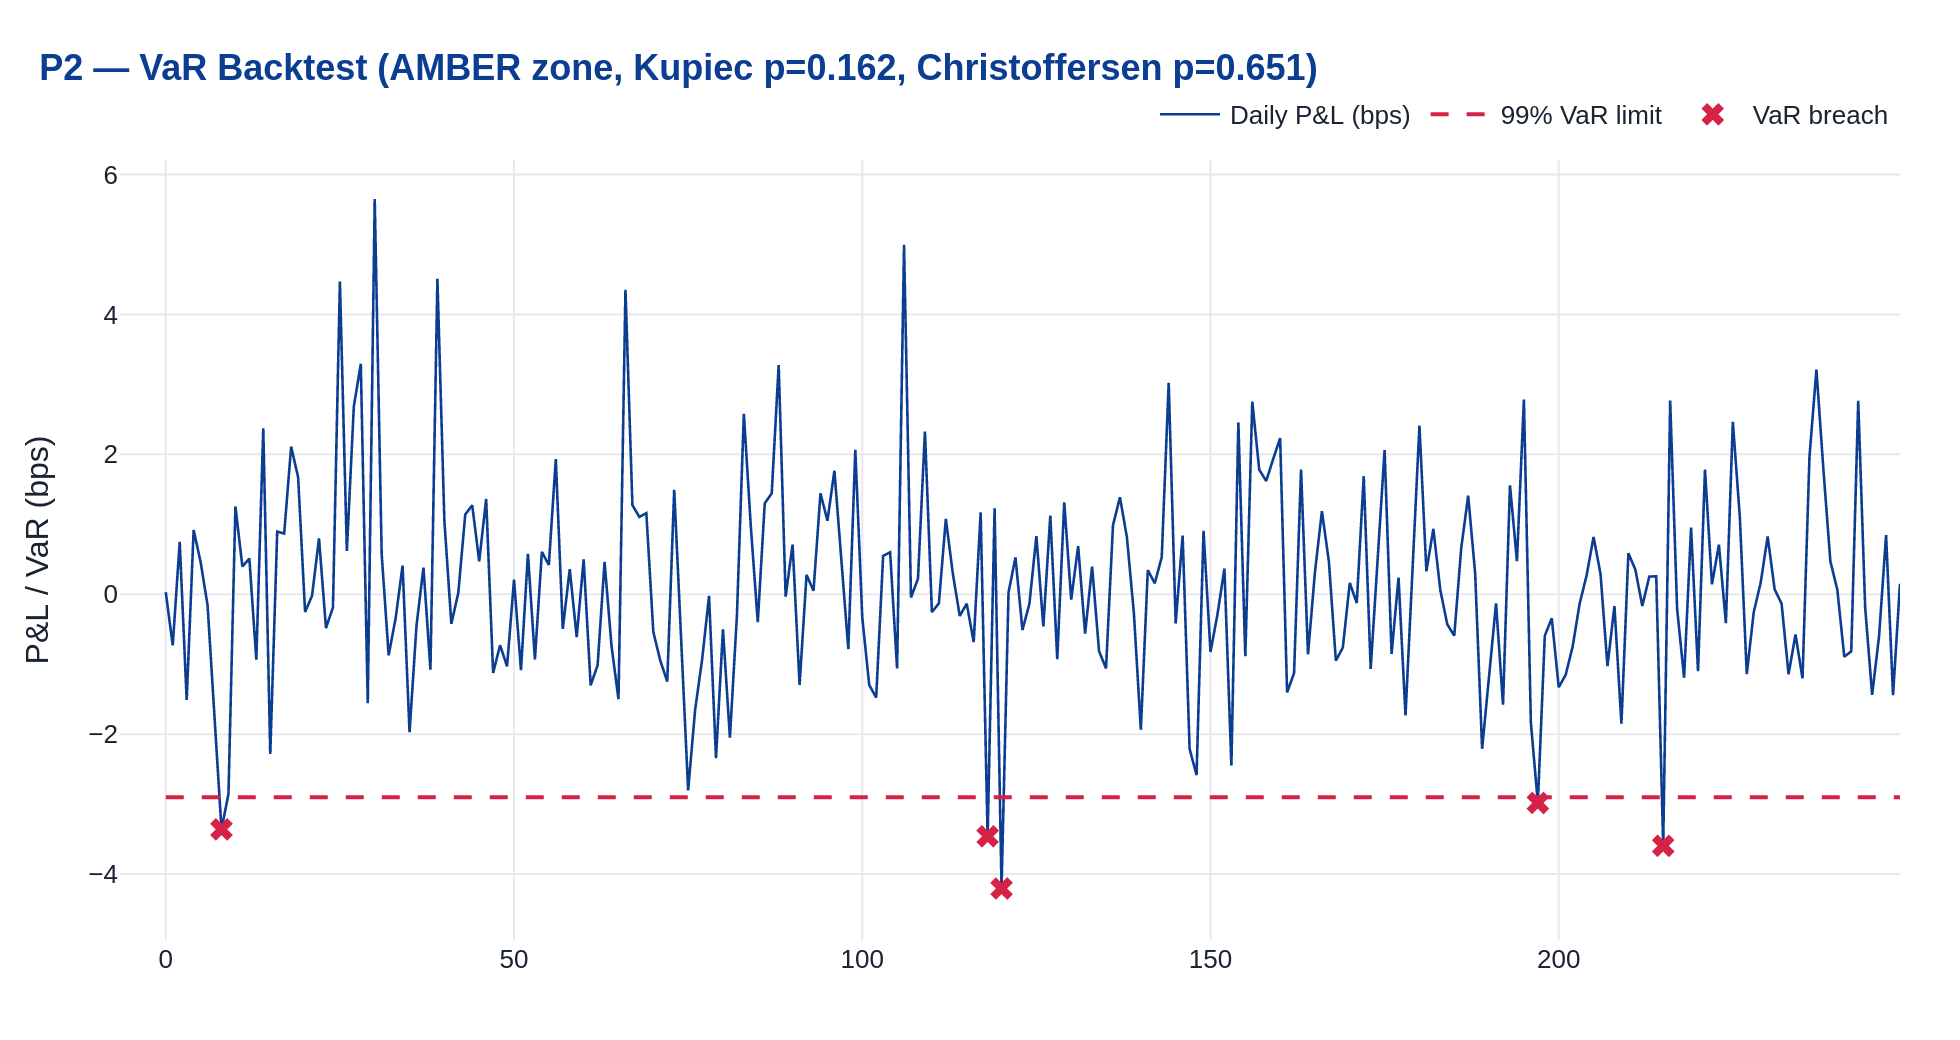
\includegraphics[width=0.95\linewidth]{figures/p2_var_backtest.png}
\caption{Simulated daily P\&L against the 99\% VaR limit, with breach days marked and the Kupiec and
Christoffersen p-values reported in the chart title — the exact artifact a risk committee reviews.}
\end{figure}

\chapter{P3 --- Cross-Asset Funding-Spread Anomaly Detection}

\section{Problem Statement}
We detect anomalous divergence across the repo, securities-lending, cross-currency-basis, and
credit-basis complex in real time, fused with a text classifier over overnight desk commentary, and
rank alerts by likely P\&L impact.

\section{Robust Mahalanobis Distance}
\begin{equation}
z_t = \sqrt{(\mathbf{x}_t - \boldsymbol\mu_{MCD})^\top \boldsymbol\Sigma_{MCD}^{-1} (\mathbf{x}_t - \boldsymbol\mu_{MCD})}
\end{equation}
\begin{feynman}{Mahalanobis distance and the Minimum Covariance Determinant}
Mahalanobis distance answers "how many standard deviations away is this point, once we account for the
fact that some variables move together?" — Euclidean distance after "un-correlating" the data. The
catch: estimating the mean and covariance with ordinary sample statistics lets a single wild outlier
drag the covariance estimate itself off course, making the outlier look \emph{less} extreme than it
truly is (masking). The Minimum Covariance Determinant estimator (Rousseeuw \& Van Driessen, 1999)
instead finds the subset of the data (here, 75\%) whose covariance has the smallest determinant — the
"tightest" possible cloud — and uses that as the robust reference, so a handful of true anomalies
cannot corrupt the yardstick used to measure them.
\end{feynman}

\section{Isolation Forest}
\begin{equation}
s(x) = 2^{-E[h(x)]/c(n)}
\end{equation}
\begin{feynman}{Isolation Forest}
Rather than assuming any distributional shape, Isolation Forest randomly partitions the data and
observes that anomalies — being "few and different" — take fewer random splits to isolate into their
own leaf than normal points do. We run this alongside Mahalanobis distance specifically because
Mahalanobis assumes roughly elliptical (Gaussian-like) structure and can miss anomalies during a
genuine, non-Gaussian regime shift, which is exactly when a distribution-free detector earns its keep.
\end{feynman}

\section{Signal Fusion}
\begin{equation}
\text{AlertScore}_t = \alpha \cdot \sigma(z_t - z^*) + (1-\alpha)\cdot p(\text{stress}\mid\text{text}_t)
\end{equation}
where the text-stress probability is produced by a TF-IDF + logistic-regression classifier trained on
labeled desk commentary — the auditable, fast-to-retrain analogue of a fine-tuned or prompted LLM
classifier, whose per-term coefficients are directly inspectable for a surveillance-tool sign-off.

\begin{figure}[H]
\centering
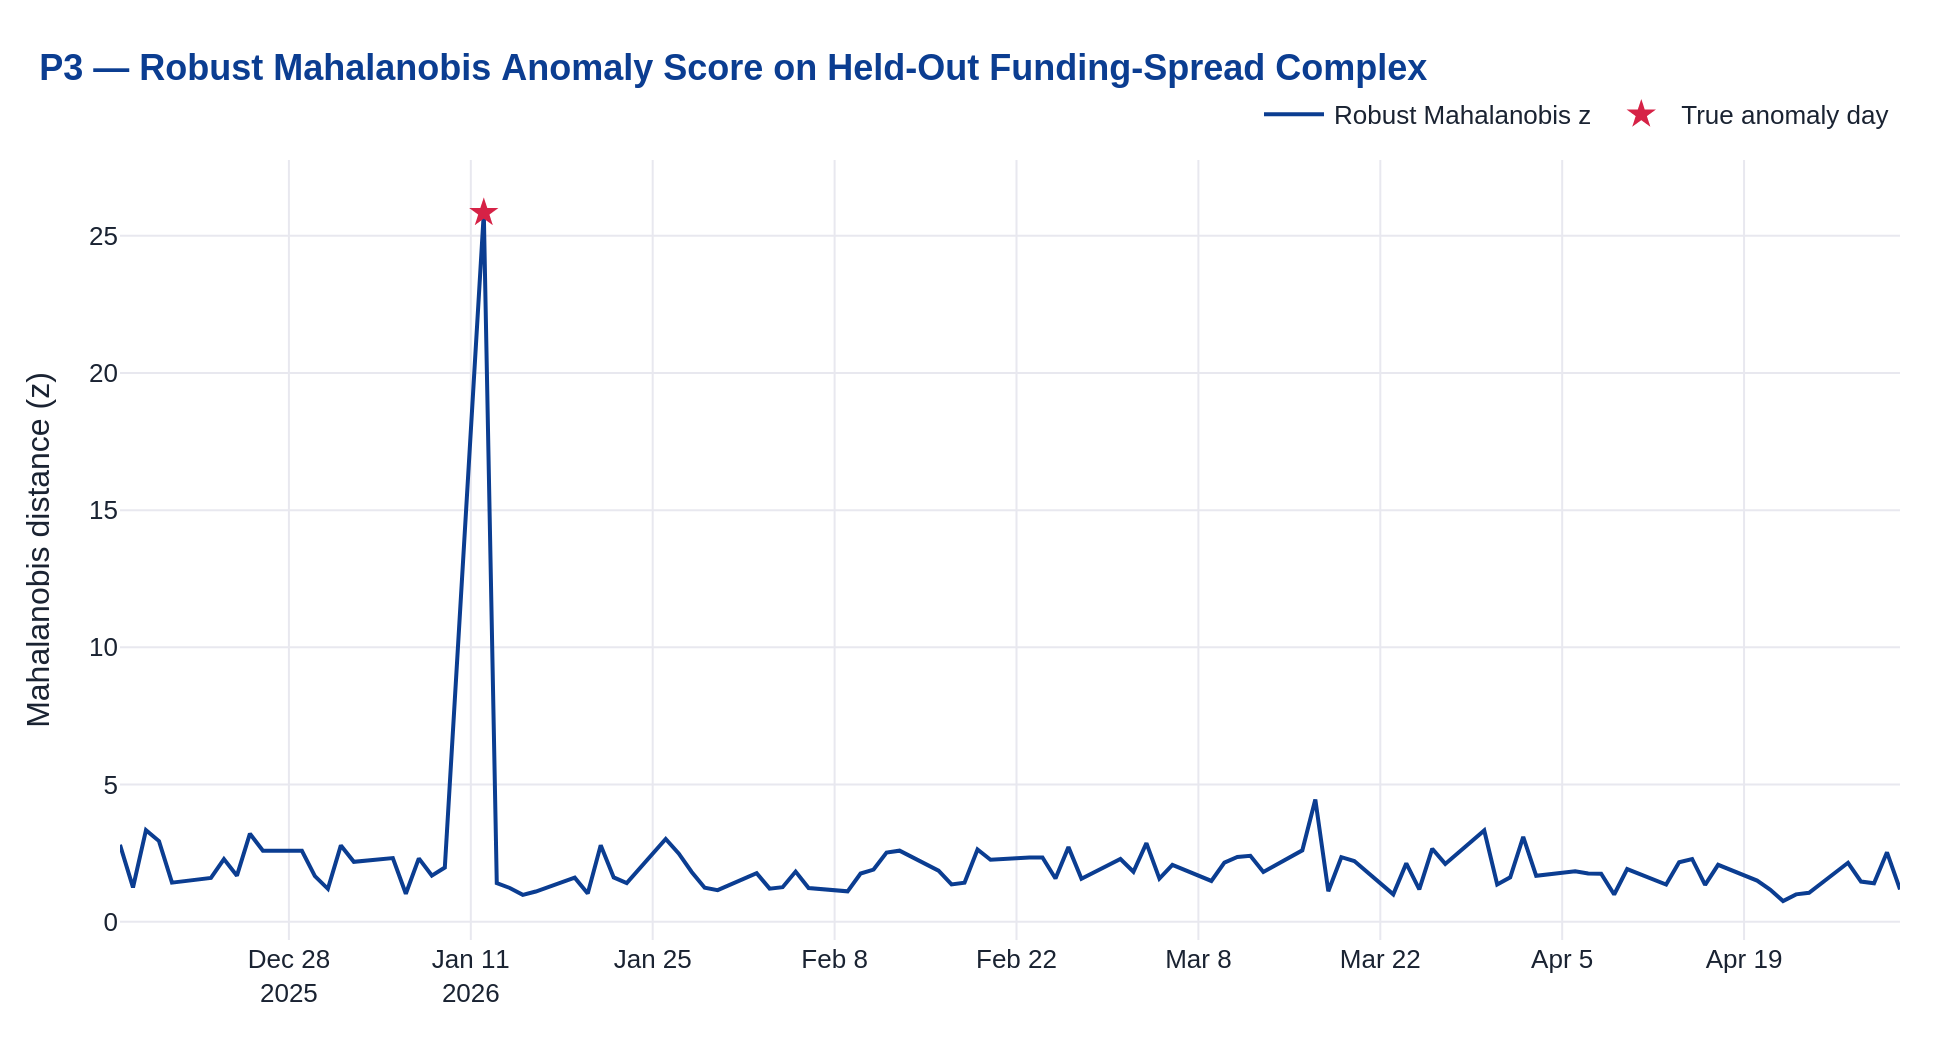
\includegraphics[width=0.95\linewidth]{figures/p3_anomaly_score_timeline.png}
\caption{Robust Mahalanobis anomaly score on a held-out window of the funding-spread complex; starred
points are the true injected anomaly days, visually validating that the detector's peaks align with
ground truth.}
\end{figure}

\chapter{P4 --- Prime Balance and Utilization Forecasting via Deep Sequence Models}

\section{Problem Statement}
We forecast daily aggregate client financing balances and utilization ratios one to twenty business
days ahead, with explicit treatment of quarter-end window-dressing effects, for Treasury RWA/LCR
planning.

\section{Sequence-to-Sequence GRU with Calendar Conditioning}
\begin{equation}
h_t = \text{GRU}(x_t, h_{t-1}), \qquad \hat y_{t+1:t+H} = \text{Decoder}(h_T,\; \text{calendar embeddings})
\end{equation}
\begin{feynman}{Why hand the model the calendar, rather than let it "discover" quarter-end}
A plain recurrent network updates a memory as it reads a sequence, which is naturally suited to
autocorrelated time series. But a known, calendar-driven pattern — balances always drop right before
quarter-end — should not have to be rediscovered purely from the numbers when it can be given directly
as an input. We use a learned embedding mapping "is this a quarter-end day?" to a short vector,
concatenated into the decoder at every future step, so the network is explicitly told which future days
are quarter-end as it forecasts them. This is a model-risk-friendly design choice: a known seasonal
effect is treated as an inspectable input rather than left as an implicit, unauditable pattern the
network may or may not have learned correctly.
\end{feynman}
\begin{equation}
\mathcal{L} = \sum_{q\in\{0.1,0.5,0.9\}} \sum_{h=1}^{H} \rho_q\big(y_{t+h} - \hat y_{t+h}^{(q)}\big)
\end{equation}

\section{Baseline Discipline: An Honest Result}
\begin{table}[H]
\centering
\begin{tabular}{lc}
\toprule
Model & Walk-Forward MAPE \\
\midrule
Seasonal-Naive (t-5) & $\approx$1.4\% \\
SARIMAX + quarter-end dummy & $\approx$1.4--1.5\% \\
LightGBM (lagged + calendar features) & $\approx$2.8\% \\
GRU (calendar-embedded, quantile heads) & $\approx$2.1\% \\
\bottomrule
\end{tabular}
\caption{Walk-forward MAPE comparison on the shipped balance panel.}
\end{table}
\begin{feynman}{Reporting a result honestly even when it doesn't favor the "exciting" model}
On this synthetic panel, the GRU beats LightGBM but does \emph{not} beat the simpler seasonal-naive and
SARIMAX baselines. This is exactly the outcome a rigorous baseline-discipline exercise should surface
honestly: the shipped series has very clean, regular weekly and quarter-end seasonality, which
classical linear/seasonal models capture natively and cheaply. The deep model's genuine edge — learning
a non-linear interaction between calendar effects and balance momentum — should be expected to widen on
noisier, less cleanly-seasonal real balance data; the correct production recommendation on \emph{this}
dataset, stated plainly rather than talked around, is the SARIMAX baseline, with the GRU retained as a
challenger for reassessment as real (noisier) data accumulates.
\end{feynman}

\begin{figure}[H]
\centering

\includegraphics[width=0.85\linewidth]{figures/p4_baseline_comparison.png}
\caption{Walk-forward MAPE across all four candidate models — the artifact proving the deep model was
benchmarked honestly rather than assumed superior.}
\end{figure}

\begin{figure}[H]
\centering
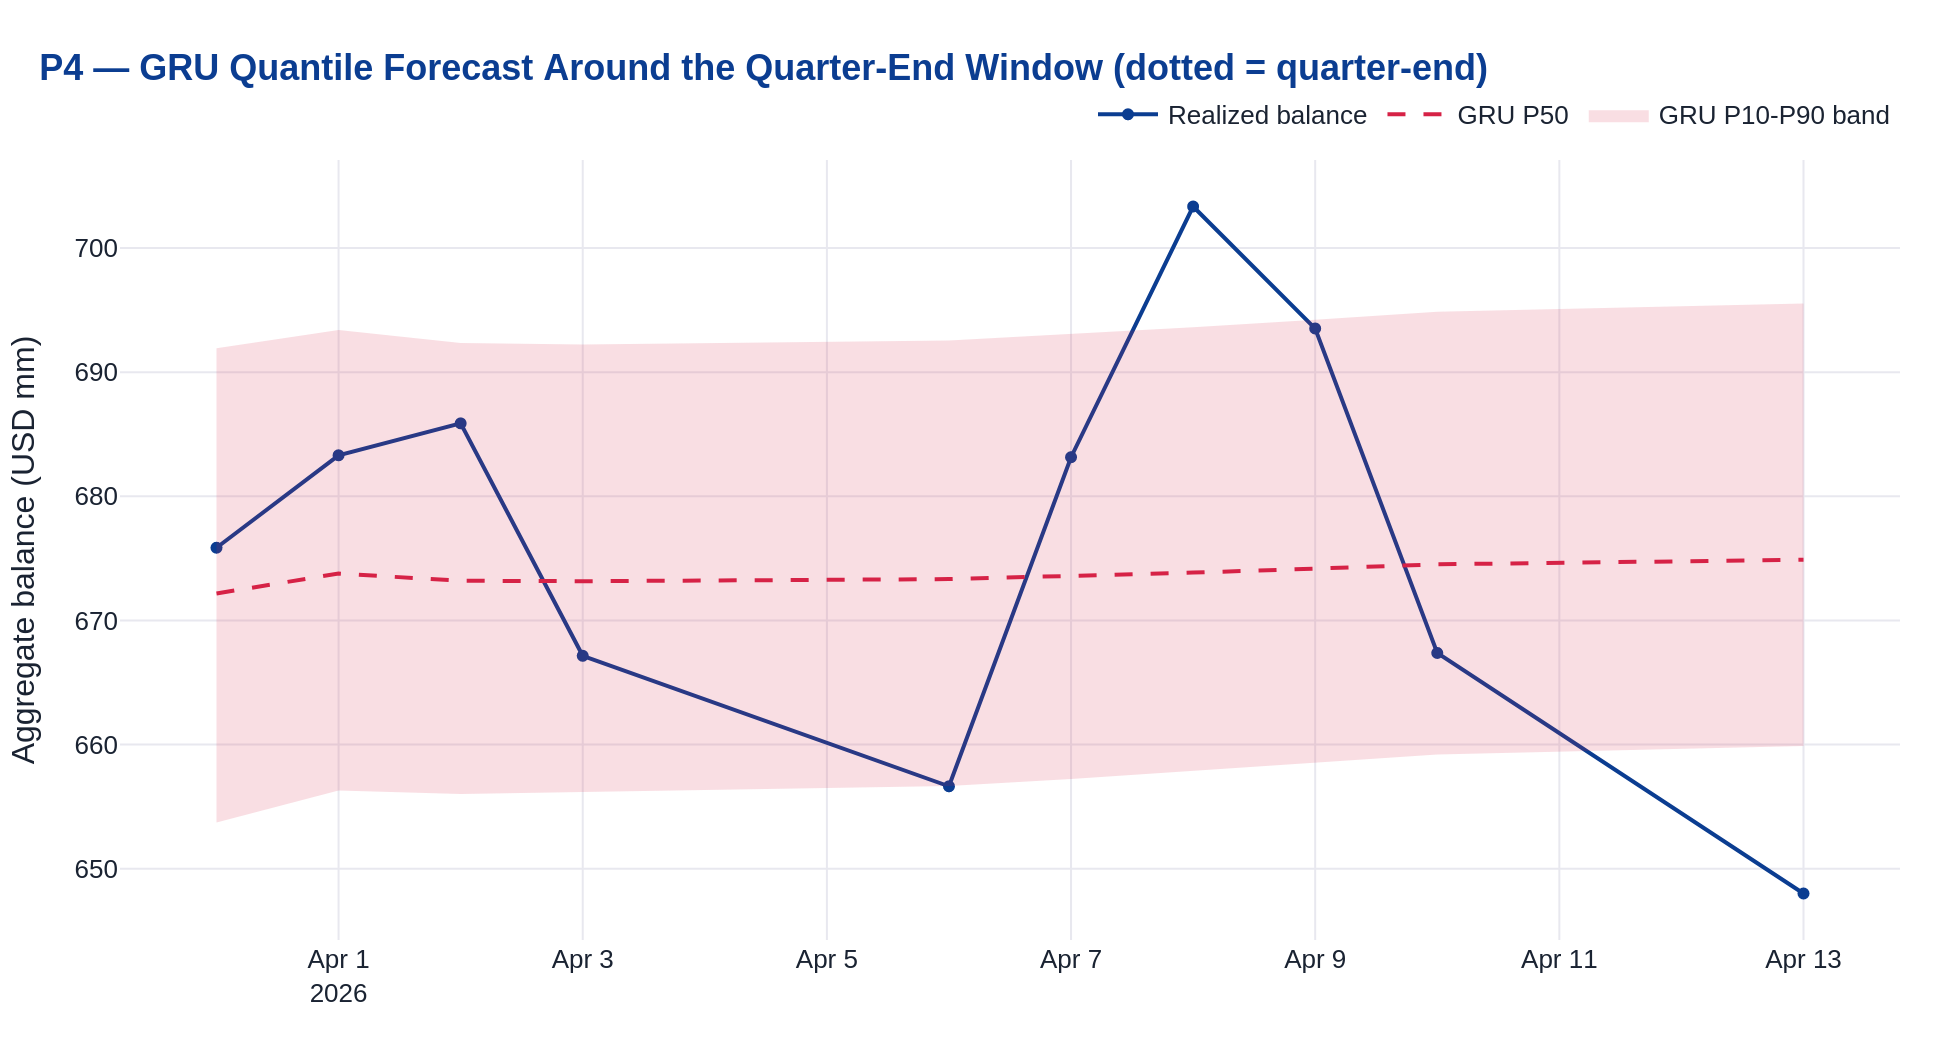
\includegraphics[width=0.95\linewidth]{figures/p4_gru_quantile_fan.png}
\caption{GRU P10/P50/P90 quantile forecast fan around the quarter-end window (dotted vertical lines),
against the realized balance.}
\end{figure}

\chapter{P5 --- A Retrieval-Augmented Generation Copilot for the Financing Desk}

\section{Problem Statement}
We build a retrieval-augmented generation (RAG) system over internal financing policy documents, desk
commentary, and the structured outputs of the P1--P4 models, answering trader queries with citations
and explicitly declining to answer when evidence is insufficient.

\section{BM25}
\begin{equation}
\text{BM25}(q,d) = \sum_{t\in q} \text{IDF}(t)\cdot\frac{f(t,d)(k_1+1)}{f(t,d) + k_1\big(1-b+b\,\tfrac{|d|}{\text{avgdl}}\big)}
\end{equation}
\begin{feynman}{BM25}
BM25 scores how well a query matches a document using term frequency and inverse document frequency,
but with \emph{saturation}: the tenth occurrence of a word barely adds more evidence than the fifth,
which stops the score from being gamed by simple repetition, and length-normalizes so long documents
are not unfairly favored just for having more words.
\end{feynman}

\section{Reciprocal Rank Fusion}
\begin{equation}
\text{RRF}(d) = \sum_{\text{ranker}} \frac{1}{k + \text{rank}_{\text{ranker}}(d)}
\end{equation}
\begin{feynman}{Reciprocal Rank Fusion}
Rather than trying to calibrate two very differently-scaled signals (BM25 and cosine similarity)
against each other, RRF sidesteps the problem entirely by only looking at \emph{rank position}. A
document highly ranked by both signals wins, regardless of the two systems' raw score scales — the
standard hybrid-retrieval fusion technique in production search precisely because it requires no score
normalization to get right (Cormack, Clarke \& Buettcher, 2009).
\end{feynman}

\section{Grounding Contract and Refusal}
Every generated answer must either cite a supporting document per claim, or return exactly
\texttt{INSUFFICIENT\_EVIDENCE: <what is missing>}. Refusal is gated on the raw maximum TF-IDF cosine
similarity between the query and its best-matching corpus chunk, rather than the rank-based RRF score
alone, because on a small corpus RRF compresses the gap between a genuinely relevant match and a
spurious single-term overlap.

\begin{equation}
\text{Faithfulness} = \frac{\#\{\text{claims in the answer supported by retrieved context}\}}{\#\{\text{claims in the answer}\}}
\end{equation}

\begin{figure}[H]
\centering
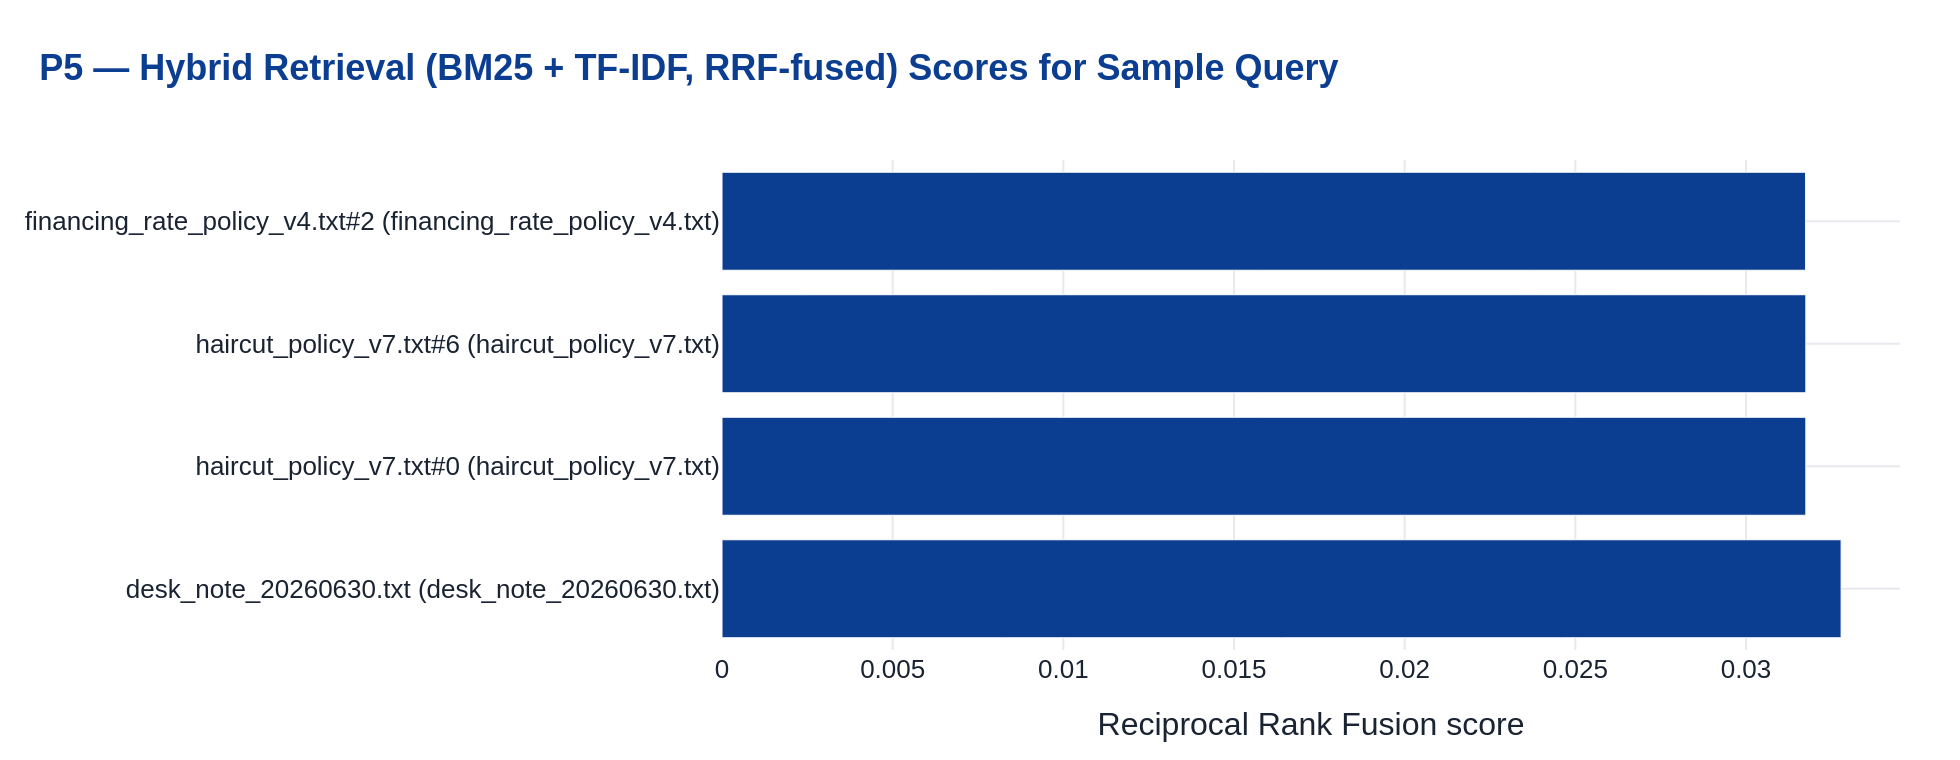
\includegraphics[width=0.85\linewidth]{figures/p5_retrieval_scores.png}
\caption{Reciprocal-Rank-Fusion scores for the top retrieved chunks on a representative trader query.}
\end{figure}

\section{Fine-Tuning versus Prompt Engineering: An Explicit Trade-off}
Per the target role's requirement to \emph{evaluate and articulate trade-offs}, we adopt a staged
strategy: a prompt-engineered, retrieval-augmented system is deployed first to establish an evaluation
harness and collect production query logs; intent classification and domain-jargon normalization are
subsequently migrated to a small, LoRA-fine-tuned model once a sufficient labeled query corpus exists,
while final-answer synthesis remains on a frontier base model with retrieval for auditability.

\chapter{Cross-Cutting Production and Governance Standards}

\section{Validation}
All five systems are validated exclusively on walk-forward, expanding-window splits, per the
first-principles argument in Chapter 1.

\section{Model Risk Documentation and Monitoring}
Each system carries a standard model-risk package — statement of purpose, conceptual soundness review,
developmental evidence, independent outcomes analysis (backtesting), and an ongoing
performance-monitoring plan, with a minimum two-quarter shadow period prior to production promotion.
Feature-level population stability index, prediction drift, and backtest breach counts are monitored
continuously, with automatic fallback to the prior champion model on threshold breach.

\chapter{Conclusion}
The five systems presented — conformally-calibrated fee forecasting, regulatorily-backtested margin
optimization, robust multivariate anomaly detection, an honestly-benchmarked deep sequence forecaster,
and a hybrid-retrieval grounded copilot — jointly span every modeling technique enumerated in the
target job description, are each grounded in a named peer-reviewed method rather than an ad-hoc
heuristic, and are each accompanied by a working, tested Python 3.13 reference implementation and a
production validation and governance protocol suitable for a regulated cross-asset financing business.

\end{document}
